% !TEX root = ../my-thesis.tex
%
\chapter{Short Introduction to Machine Learning}\label{ch:ml}
Machine learning is a generic term for the "artificial" generation of knowledge from experience: an artificial system learns from examples and can generalize these after the learning phase is complete. To do this, machine learning algorithms build a statistical model based on training data. This means that the examples are not simply learned by heart, but patterns and regularities are recognized in the learning data. In this way, the system can also assess unknown data or fail to learn unknown data. This chapter gives a short overview over some commonly used algorithms in machine learning and show how these can be optimized using hyperparameter tuning. A relatively new area of machine learning, interpretable machine learning, and some of the methods used in this area are introduced in the final parts of the chapter.
\section{Common Machine Learning Algorithms}\label{sec:algo}
In the following sections, the algorithms that are used to compute the predictive models in Section~\ref{sec:predictive} are introduced.
\subsection{K-Nearest Neighbours}
The k-nearest neighbour algorithm (knn) is a non-parametric method in which class assignment is performed considering the $k$ nearest neighbours. \\
In the simplest case, the classification of an object $x\in\mathbb{R}^n$ is done by majority vote. The $k$ nearest already classified objects of $x$ participate in this voting. To determine which neighbour is closest, many distance measures can be used. Among the most common is the Euclidean distance, defined as
\begin{equation}
    d\left(x,y\right)=\left|\left|x-y\right|\right|=\sqrt{\sum_{i=1}^n\left(x_i-y_i\right)^2}
\end{equation}
\autocite[][]{danielsson1980euclidean}.\\
Another commonly used distance metric is the Manhattan distance, which defines the distance $d$ between two points $x$ and $y$ as the sum of the absolute difference of the individual coordinates or features,
\begin{equation}
    .d\left(x, y\right) = \sum_{i=1}^n\left|x_i-y_i\right|
\end{equation}
\autocite[][]{krause1986taxicab}. \\
$x$ is assigned to the class that occurs most frequently among the $k$ neighbours. To avoid ties between two classes, an odd value can be chosen for $k$. 
If the value of $k$ is small, there is a risk that noise in the training data can lead to worse classification results, while a value that is too large risks including points with a large distance to $x$ in the decision. \\
The algorithm can be used for regression problems to estimate continuous variables. While in knn classification the output is the class membership, in knn regression the output is the average value of the $k$ nearest neighbours \autocite[][]{altman1992introduction}
\subsection{Neural Networks}
Artificial neural networks, usually referred to simply as neural networks, are computer systems vaguely inspired by the biological neural networks that make up the brains of living things. Neural networks, however, are more about an abstraction (modelling) of information processing, less about replicating biological neural networks and neurons, which is more the subject of computational neuroscience. Motivated by biology, modelling is now so good that many tasks are performed much better than by humans. \\
In artificial neural networks, topology refers to the structure of the network. This generally means how many artificial neurons are located on how many layers and how they are connected to each other. Artificial neurons can be connected in many ways to form an artificial neural network. In many models, neurons are arranged in layers; a network with only one trainable neuron layer is called a single-layer network. 
Using a graph, the neurons can be represented as nodes and their connections as edges. The inputs are occasionally represented as nodes. 
The backmost layer of the network, whose neuron outputs are usually the only ones visible outside the network, is called the output layer. Layers before this are referred to as the hidden layer. Figure~\ref{fig:nnet} shows the architecture of a single-layer neural network.
\begin{figure}[H]
    \centering
    \def\layersep{2.5cm}

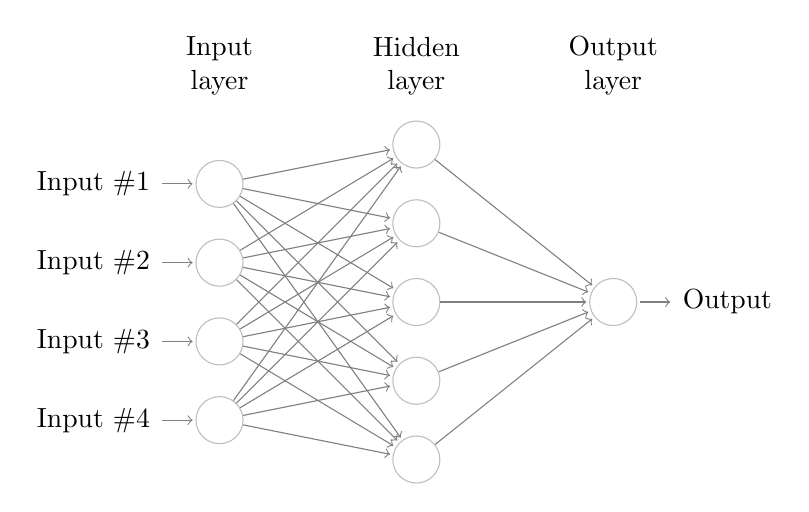
\begin{tikzpicture}[shorten >=1pt,->,draw=black!50, node distance=\layersep]
    \tikzstyle{every pin edge}=[<-,shorten <=1pt]
    \tikzstyle{neuron}=[circle,fill=black!25,minimum size=17pt,inner sep=0pt, draw=black!25]
    \tikzstyle{input neuron}=[neuron, fill=white!50];
    \tikzstyle{output neuron}=[neuron, fill=white!50];
    \tikzstyle{hidden neuron}=[neuron, fill=white!50];
    \tikzstyle{annot} = [text width=4em, text centered]

    % Draw the input layer nodes
    \foreach \name / \y in {1,...,4}
    % This is the same as writing \foreach \name / \y in {1/1,2/2,3/3,4/4}
        \node[input neuron, pin=left:Input \#\y] (I-\name) at (0,-\y) {};

    % Draw the hidden layer nodes
    \foreach \name / \y in {1,...,5}
        \path[yshift=0.5cm]
            node[hidden neuron] (H-\name) at (\layersep,-\y cm) {};

    % Draw the output layer node
    \node[output neuron,pin={[pin edge={->}]right:Output}, right of=H-3] (O) {};

    % Connect every node in the input layer with every node in the
    % hidden layer.
    \foreach \source in {1,...,4}
        \foreach \dest in {1,...,5}
            \path (I-\source) edge (H-\dest);

    % Connect every node in the hidden layer with the output layer
    \foreach \source in {1,...,5}
        \path (H-\source) edge (O);

    % Annotate the layers
    \node[annot,above of=H-1, node distance=1cm] (hl) {Hidden layer};
    \node[annot,left of=hl] {Input layer};
    \node[annot,right of=hl] {Output layer};
\end{tikzpicture}
    \caption{A single-layer neural network.}
    \label{fig:nnet}
\end{figure}
While neural networks are mainly known for their use in deep learning and modelling complex problems such as image recognition, they can be easily adapted for regression problems. In supervised learning, the neural network is given an input pattern and the output produced by the neural network in its current state is compared with the value it is supposed to output. By comparing the target and actual output, it is possible to infer the changes to be made to the network configuration \autocite[][]{ripley2007pattern}.
\subsection{Classification and Regression Trees}
Classification and regression trees (CART) is an approach to classification or regression problems. A significant feature of the CART algorithm is that only binary trees can be generated, which means that there are always exactly two branches at each node. The central element of this algorithm is therefore finding an optimal binary separation.
In the CART algorithm, attribute selection is controlled by maximizing the information content. CARTs are characterized by optimally separating the data in terms of classification. This is achieved with a threshold value that is searched for each attribute. The information content of an attribute is considered high if a classification can be made with a high hit rate by evaluating the attribute characteristics resulting from the division via the threshold values. For the decision trees calculated by the CART algorithm, the following applies: The higher the information content of an attribute in relation to the target variable, the higher up in the tree this attribute is found. Figure~\ref{fig:tree} shows an example of a decision tree.
\begin{figure}[H]
    \centering
    \begin{tikzpicture}[
    node/.style={%
      draw,
      rectangle,
    },
  ]

    \node [node] (A) {Carbohydrates > 20};
    \path (A) ++(-135:\nodeDist) node [node] (B) {Brunost};
    \path (A) ++(-45:\nodeDist) node [node] (C) {Fett > 25};
    \path (C) ++(-135:\nodeDist) node [node] (D) {Gulost};
    \path (C) ++(-45:\nodeDist) node [node] (E) {Gräddost};

    \draw (A) -- (B) node [left,pos=0.25] {yes}(A);
    \draw (A) -- (C) node [right,pos=0.25] {no}(A);
    \draw (C) -- (D) node [left,pos=0.25] {no}(A);
    \draw (C) -- (E) node [right,pos=0.25] {yes}(A);
\end{tikzpicture}
    \caption{A simple example of a decision tree}
    \label{fig:tree}
\end{figure}
In regression analysis, trees are built by a collection of rules based on the available features of the dataset:
\begin{itemize}
    \item Rules based on the values of the variables are selected to obtain the best split to distinguish the observations based on the dependent variable.
    \item Once a rule is selected and a node is split into two parts, the same process is applied to each "child" node (i.e. it is a recursive process).
    \item Splitting stops when the algorithm determines that no further gain can be made or when some preset stop rules are met. (Alternatively, the data is split as much as possible and the tree is pruned later).
\end{itemize}
Each branch of the tree culminates in a terminal node. Each observation falls into exactly one terminal node, and each terminal node defined by a unique set of rules \autocite[][]{breiman1984classification}.
\subsection{Gradient Boosting}
CART are considered weak learners, meaning that their predictive performance is only slightly better than chance. Boosting is a method that can be used to convert weak learners into strong learners. Gradient boosting in particular uses CART as a weak learner. Here, each new tree is an adaptation to a modified version of the original tree. After the first tree is grown, the error residuals, defined as the difference between the target value and the predicted target value, are calculated. A new tree is fitted using the error residuals as the target variable while still using the same input variables. The predicted residuals are added to the previous predictions. This procedure is repeated for the remaining residuals until the loss reaches an acceptable level or no longer improves on an external validation set. \\
Trees are added one at a time and existing trees in the model are not changed. After calculating the loss, a tree must be added that reduces the loss (i.e. follows the gradient). The mathematical version of the algorithm can be seen in Algorithm~\ref{alg:gradient}.
\begin{algorithm}[H]
\caption{The Gradient Boosting Algorithm}
  \label{alg:gradient}
\begin{algorithmic}[1]
\Statex Given a training set $\lbrace\left(x_i,y_i\right)\rbrace_{i=1}^n$, a differentiable loss function $L\left(y, F(x)\right)$ and the number of iterations $M$,
\State Initialization: Compute a model with a constant value:
\begin{equation*}
    F_0\left(x\right)=\underset{\gamma}{\arg\min}\sum_{i=1}^nL\left(y_i,\gamma\right).
\end{equation*}
\For{each iteration $m=1$ to $M$}
    \State Compute \textit{pseudo-residuals}:
    \begin{equation*}
        r_{im}=-\left[\frac{\partial L\left(y_i, F\left(x_i\right)\right)}{\partial F\left(x_i\right)}\right]_{F(x)=F_{m-1}(x)}, \hspace{10pt}\hbox{for } i=1,...,n.
    \end{equation*}
    \State Fit a weak learner $h_m(x)$ to the pseudo-residuals, using $\lbrace\left(x_i,r_{im}\right)\rbrace_{i=1}^n$ as the training set 
    \State Compute the multiplier $\gamma_m$ by solving the following optimization problem:
    \begin{equation*}
        \gamma_m=\underset{\gamma}{\arg\min}\sum_{i=1}^nL\left(y_i,F_{m-1}\left(x_i\right)+\gamma h_m\left(x_i\right)\right).
    \end{equation*}
    \State Update the model:
    \begin{equation*}
        F_m\left(x\right)=F_{m-1}(x)+\gamma_mh_m(x).
    \end{equation*}
    \EndFor
\State Output: $F_M(x)$
\end{algorithmic}
\end{algorithm} $\newline$
Gradient boosting of CART produces robust and interpretable models for both regression and classification that achieve high predictive accuracy \autocite[][]{friedman2001greedy}.
\subsection{Random Forests}
A Random Forest is a classification and regression procedure consisting of several uncorrelated decision trees. All decision trees are grown under a certain type of randomization during the learning process. For a classification, each tree in that forest is allowed to make a decision and the class with the most votes decides the final classification. Random forests can be used for regression. Random forest uses bagging, a meta-algorithm that can be used to improve the stability and accuracy of machine learning algorithms, for instance CART. \\
Using $B$ samples of size $n$, $B$ models $F_i(x), i = 1,..., B$ are computed. For each $x$, $B$ predictions $m_{i}(x), i = 1,...B$ exist then. The predicted value is given by
\begin{equation}
    m^B(x)=\frac{1}{B}\sum_{i=1}^B\left(m_i(x)\right).
\end{equation}
This method, as well as random forest, were both developed by Leo Breiman \autocite[][]{breiman1996bagging}. Random forests differ in only one way from this general scheme: they use a modified tree learning algorithm that selects, at each candidate split in the learning process, a random subset of the features. This process is sometimes called "feature bagging". The reason for doing this is the correlation of the trees in an ordinary bootstrap sample: if one or a few features are strong predictors for the response variable (target output), these features are selected in many of the $B$ trees, causing them to become correlated. A general overview of the random forest is given in Algorithm~\ref{alg:rf}
\begin{algorithm}[H]
\caption{The Random Forest Algorithm}
  \label{alg:rf}
\begin{algorithmic}[1]
\Statex Given a training set $\lbrace\left(x_i,y_i\right)\rbrace_{i=1}^n$, the number of trees $B$ and the number of variables $m$ that should be tried at each split
\State Draw $B$ bootstrap-samples of $\lbrace\left(x_i,y_i\right)\rbrace_{i=1}^n$
\State From the $M$ features of the training data, $m \ll M$ features are randomly selected at each node in the tree to be considered as criteria for the cut (split).
\State Each tree is fully grown and not pruned back
\end{algorithmic}
\end{algorithm} $\newline$
To classify an input, it is evaluated in each tree. The class that is chosen most often is the output of the random forest. In the case of regression, the average prediction is used \autocite[][]{breiman2001random}
\clearpage
\section{Machine Learning Methodology}\label{sec:methods}
After introducing some common machine learning algorithms, this section shows how these algorithms can be optimized to achieve the best possible performance with respect to a given performance measure. Even though machine learning models are often referred to as "black boxes", there are methods to make these models more interpretable. These are presented in this section as well.
\subsection{Tuning of Machine Learning Models}
In the field of machine learning, hyperparameter optimization, also known as hyperparameter tuning, refers to the search for optimal hyperparameters. A hyperparameter is a parameter that is used to control the training algorithm and whose value, unlike other parameters, must be set before the actual training of the model. There exists a variety of methods when it comes to the algorithms used to explore the hyperparameter space, from simple methods like a grid search to Bayesian optimization or more advanced methods like iterated F-racing.
\subsubsection*{Cross-Validation}
Cross-validation is a procedure for evaluating the performance of an algorithm in machine learning. Using new datasets that were not used during the training phase, the goodness of the prediction is examined. This is done by partitioning the known dataset into subsets for training and testing the algorithm and the remaining data.
Each run of cross-validation involves randomly partitioning the original dataset into a training set and a test set. The training data set is used to train a supervised learning algorithm and the test data set is used to evaluate its performance. This process is repeated several times and the mean cross-validation error is used as a performance indicator.
When training a model, it is important not to overfit it with complex algorithms or underfit it with simple algorithms. The choice of training and testing set is critical to reducing this risk. However, it is difficult to split the dataset in a way that maximizes learning and the validity of the test results. This is where cross-validation comes in. To find the best algorithm for the model, cross-validation offers different techniques that split the data differently. \\
A commonly used cross-validation procedure is k-fold cross-validation. In this method, after splitting the original dataset into a training and a test dataset, the training set is split into $k$ subsets called folds. Cross-validation iterates through each fold, using one of the $k$ folds as the validation set at each iteration, while all the remaining folds are used as the training set. This process is repeated until every fold has been used as a validation set. \\
Cross-validation helps to select the best performing model by calculating the error using the test set that is not used for training. The test set is used to calculate model accuracy and show how it generalizes with future data \autocite[][]{fushiki2011estimation}. Figure~\ref{fig:cv} shows an example of 10-fold cross validation.
\begin{figure}[H]
    \centering
    \begin{tikzpicture}[node distance=0mm,minimum height=1cm,outer sep=3mm,scale=0.4,>=Latex,font=\footnotesize,
  indication/.style={minimum height=0cm,outer sep=0mm},
  oneblock/.style={transform shape,minimum width=1cm,draw},
  fullset/.style={transform shape,minimum width=10cm,draw}]
    % left part of picture
    \node[fullset,anchor=west] at (0,0) (A) {};
    \node[above=of A.north,indication] (ATXT) {TRAINING SET};
    \node[oneblock,minimum width=2cm,anchor=west,right=of A,fill=lightgray,outer sep=0mm] (A1) {};
    \path (ATXT) -| (A1) node[midway] {TEST SET};
    \node[fullset,anchor=west] at (0,-4) (B) {};
    \foreach \x in {0,1,...,9}
    {
        \draw (B.west) +(\x,0) node[oneblock,anchor=west,draw] {};
    }
    \draw[->] (A) -- (B) node[midway,fill=white,indication] {divide into 10 folds of equal size};

    % right part of picture
    \begin{scope}[xshift=15cm,scale=0.5,local bounding box=rightside box]
    \foreach \x in {0,1}
    {
        \foreach \y in {0,1,...,4}
        {
            \draw (\x*11,0) +(0,-\y*1) node[fullset,anchor=west] {};
            \draw (\x*11,0) +(\x*5+\y,-\y*2) node[oneblock,draw,anchor=west,fill=lightgray] {};
        }
    }
    \coordinate (R) at (rightside box.west);
    \end{scope}

    % connecting arrow
    \draw[->] (B.east) -- +(2.5,0) node[below,align=center,indication] {run experiments\\using 10 different\\partitionings} |- (R);
  \end{tikzpicture}
    \caption{An example of 10-fold cross validation}
    \label{fig:cv}
\end{figure}
\subsubsection*{Grid and Random Search}
The two most commonly used methods for hyperparameter tuning are grid search and random search. Grid search performs an exhaustive search on a manually defined subset of the learning algorithm's hyperparameter space. A grid search must be guided by a performance metric, typically computed by cross-validation on training data or validation data that is not considered during training. For example, for a knn algorithm, a grid search may try any value for $k$ between 1 and 20 and return the best value for $k$ with respect to a performance measure. One of the major disadvantages of grid search is that it suffers in terms of dimensionality when the number of hyperparameters grows exponentially. With only four parameters, this problem can become impractical as the number of evaluations required for this strategy increases exponentially with each additional parameter due to the curse of dimensionality. \\
In the random search, instead of exhaustively trying all combinations, a random selection of values is made within the given hyperparameter space. Unlike grid search, no discretization of the space is required. Random search can outperform grid search in speed and performance, especially when only a few hyperparameters affect the quality of the learning algorithm. This is because grid search tries only a few values for each parameter (but multiple times), while randomly selected values are much better distributed in the search space \autocite[][]{bergstra2012random}.
\subsubsection*{F-Race and Iterated F-Racing}
F-Race is a racing algorithm that is used to select the best configuration of parameterized algorithms based on statistical approaches. The main idea is to iteratively evaluate a given finite set of candidates on a stream of instances. After each iteration, some candidate configurations that perform significantly worse than others under the Friedman test with post-hoc analysis for pairs are eliminated and only the remaining ones are evaluated for subsequent iterations. The Friedman test is a statistical test for examining three or more paired samples for equality of the location parameter. \\
As this process continues, this method focuses more and more on the most promising candidate configurations. An essential part in F-Race is defining the set of candidate configurations of the first step. One way is iterated F-Race, which creates a probability model for a candidate solution. A set of candidates is evaluated at each iteration to update the probability model and steer the next sample towards the better candidate solutions until a termination criterion is met \autocite[][]{birattari2010f}.
\subsection{Interpretation of Machine Learning Models}
After creating a model, possibly tuning its hyperparameters and finally training it, the logical next step would be to make predictions for unseen data. The accuracy of the predictions can be evaluated using a performance measure such as the mean absolute error. Beyond that, however, it is often quite difficult to interpret the final model or get an idea of why it predicts a particular value given a set of input variables. This is where interpretable machine learning (IML) comes in, as it aims to shed more light into the black box that is most machine learning algorithms.
\subsubsection*{Feature Importance}
The idea behind feature importance is simple. The importance of a feature is measured by calculating the increase in the model's prediction error after permuting the feature. The more the model error is increased by this permutation, the more important a feature is, as this means that the model relies on the feature for prediction. If the model error does not change, a feature is unimportant because the model ignored the feature for prediction. Algorithm~\ref{alg:importance} shows how the algorithm works in practice.
\begin{algorithm}[H]
\caption{The Permutation Feature Importance Algorithm}
  \label{alg:importance}
\begin{algorithmic}[1]
\Statex Given a trained model $F$, a feature matrix $\pmb{X}$, a target vector $\pmb{y}$ and a loss function $L\left(\pmb{y}, F\right)$
\State Estimate the original model error $\varepsilon_{\hbox{\footnotesize orig}}=L\left(\pmb{y}, F(\pmb{X})\right)$
\For{each feature $j=1,...,p$}
    \State Generate permuted feature matrix $\pmb{X}_{\hbox{\footnotesize perm}}$ by permuting feature $j$ in the data $\pmb{X}$, thereby breaking the association between $j$ and the outcome $\pmb{y}$.
    \State Calculate the permutation error $\varepsilon_{\hbox{\footnotesize perm}}=L\left(\pmb{y}, f\left(\pmb{X}_{\hbox{\footnotesize perm}}\right)\right)$ based on the predictions of the permuted data.
    \State Calculate the permutation feature importance $FI_j=\frac{\varepsilon_{\hbox{\footnotesize perm}}}{\varepsilon_{\hbox{\footnotesize orig}}}$.
    \EndFor
\State Sort the features by descending $FI$.
\end{algorithmic}
\end{algorithm} $\newline$
The advantages of feature importance include that it is easy to interpret, it is comparable across different problems, it accounts for all interactions, and it does not require retraining of the model. On the other hand, there is no clear guideline whether it should be used for training or testing data, the true outcome must be known, and the measurement may be biased if the features are correlated \autocite[][]{fisher2018model, molnar2020interpretable}.
\subsubsection*{Partial Dependence Plots}
The partial dependence plot (PDP) shows the marginal effect that one or two features have on the predicted outcome of a machine learning model. A partial dependence plot can reveal whether the relationship between the dependent value and a feature is linear, monotonic or more complex. When applied to a linear regression model, for example, partial dependence plots show a linear relationship every time. \\
For regression, the partial dependence function is given by
\begin{equation}
    \widehat{f}_{\pmb{x}_S}\left(\pmb{x}_S\right)=\mathbb{E}_{\pmb{x}_C}\left[\widehat{f}\left(\pmb{x}_S, \pmb{x}_C\right)\right] = \int\widehat{f}\left(\pmb{x}_S,\pmb{x}_C\right)d\mathbb{P}\left(\pmb{x}_C\right).
\end{equation}
$\pmb{x}_S$ denotes the features for which the partial dependence function is to be plotted and $\pmb{x}_C$ denotes the rest of the features used in the model $\widehat{f}$. In general, the set $S$ contains only one or two features and these are the ones for which the effect on the prediction is to be evaluated. The total feature space $\pmb{x}$ is composed of the feature vectors $\pmb{x}_S$ and $\pmb{x}_C$. By marginalizing the output of $\widehat{f}$ over the distribution of the features in set $C$, the function shows the relationship between the features in $S$ and the predicted outcome. This process produces a function that depends only on the features in $S$ and includes interactions with other features. \\
$\widehat{f}_{\pmb{x}_S}$ is estimated by averaging the training data,
\begin{equation}
    \widehat{f}_{\pmb{x}_S}\left(\pmb{x}\right)=\frac{1}{n}\sum_{i=1}^n\widehat{f}\left(\pmb{x}_S, x_{C, i}\right).
\end{equation}
For given value(s) of $S$, the function returns the average marginal effect on the prediction. $x_{C,i}$ denotes the feature values from the dataset for the features not of interest and $n$ denotes the number of observations in the dataset. For a PDP, it is assumed that the features in $C$ and the features in $S$ are not correlated. Violation of this assumption leads to improbable or impossible data points for the PDP. \\
The advantages of PDPs include clear interpretation and intuitiveness of the method, as the partial dependence function at a given feature value represents the average prediction when all data points are forced to assume that feature value. \\
Disadvantages include the aforementioned assumption of independence and that a maximum of two features can realistically be used, as more than three dimensions are inconceivable to humans \autocite[][]{friedman2001greedy, molnar2020interpretable}.
\subsubsection*{Individual Conditional Expectation}
The PDP for the average impact of a feature is a global method as it does not focus on specific instances but on a total average. The equivalent of a PDP for individual instances of data is called an individual conditional expectation (ICE) plot. An ICE plot visualizes the dependence of the prediction on a feature for each instance separately, leading to one line per instance, compared to the one line in PDPs. Hence, a PDP represents the average of the lines in an ICE plot. The values relating to a line (and one instance) are calculated by keeping the rest of the features the same, producing variants of that instance by replacing the value of the feature with values from a grid, and making predictions using the model for these newly created instances. This results in a set of points for an instance with the feature value from the grid and the respective predictions. \\
Since a PDP only displays the average relationship between a feature and the prediction, heterogeneous relationships arising from interactions can be hidden. If the interactions between the features for which the PDP is calculated and the other features are weak, this is not a problem. However, if these interactions are not weak, an ICE plot provides deeper insight.\\
Formally, for each instance in $\lbrace\left(x_{S,i}, x_{C,i}\right)\rbrace_{i=1}^N$, $\widehat{f}_{S,i}$ is plotted against $x_{S,i}$, where $x_{C,i}$ remains fixed.\\
ICE curves are even more intuitive than a PDP, with each line representing the predictions for an instance when the feature of interest is varied. In addition, they can reveal heterogeneous relationships. \\
Drawbacks include the fact that only one display can be meaningfully plotted, as plotting multiple lines would require drawing multiple overlapping surfaces that would make it difficult to see anything in the plot. It is difficult to see the average and there may be crowding in the plot if too many lines are drawn \autocite[][]{goldstein2015peeking, molnar2020interpretable}
\subsubsection*{Shapley Values}
A prediction can be explained with the assumption that each feature value of the instance is a "player" in a game where the prediction is the payout. A fair distribution of the "payout" among the individual features can be obtained using Shapley values - a methodology from coalitional game theory. The Shapley value, is a method that assigns payouts to players depending on how much they contributed to the total payout. Players cooperate in a coalition and as a result receive a certain profit from this coalition. \\
In machine learning, the "game" is a prediction task for a single observation of the dataset. The difference between the actual prediction of this observation and the average prediction of all instances is the "gain". Feature values of the observation represent the "players" that cooperate to obtain the gain, i.e. to predict a certain value. The Shapley value is thus the average marginal contribution of the value of a feature across all possible coalitions. \\
The Shapley value is given by a value function of the players in $S$. For a single feature value, the Shapley value is its contribution to the payoff, weighted and summed over all possible feature value combinations,
\begin{equation}
    \phi_j\left(\hbox{val}\right)=\sum_{S\subseteq \lbrace x_1,...,x_p\rbrace\setminus \lbrace x_j\rbrace}\frac{\left|S\right|!\left(p-\left|S\right|-1\right)!}{p!}\left(\hbox{val}\left(S\cup\lbrace x_j\rbrace\right)-\hbox{val}(S)\right).
\end{equation}
$S$ denotes a subset of the features used in the model, $\pmb{x}$ is the vector of feature values of the instance to be explained and $p$ stands for the number of features. $\hbox{val}_x(S)$ denotes the prediction for the feature values in $S$ marginalized over features excluded from $S$,
\begin{equation}
    \hbox{val}_{\pmb{x}}(S)=\int\widehat{f}\left(x_1,...,x_p\right)d\mathbb{P}_{\pmb{x}\notin S} - \mathbb{E}_{\pmb{X}}\left[\widehat{f}(\pmb{X})\right].
\end{equation}
In practice, multiple integrations are performed for each feature that is not included in $S$. \\
The definition of a fair allocation can be viewed as an allocation that has four properties: Efficiency, Symmetry, Dummy and Additivity. The only allocation method that satisfies these four properties is the Shapley value. \\
\textbf{Efficiency}: The contributions of the individual features must add up to the difference between the prediction for $\pmb{x}$ and the average prediction,
\begin{equation*}
    \sum_{j=1}^p\phi_j=\widehat{f}(\pmb{x})-\mathbb{E}_{\pmb{X}}\left[\widehat{f}(\pmb{X})\right].
\end{equation*}
\textbf{Symmetry}: Two characteristic values $j$ and $k$ should have the same contribution if their contribution to all possible coalitions is the same. Consequently, if
\begin{equation*}
    \hbox{val}\left(S\cup\lbrace x_j\rbrace\right) = \hbox{val}\left(S\cup\lbrace x_k\rbrace\right)\hspace{10pt}\forall S\subseteq\lbrace x_1,...,x_p\rbrace\setminus\lbrace x_j,x_k\rbrace,
\end{equation*}
then
\begin{equation*}
    \phi_j=\phi_k.
\end{equation*}
\textbf{Dummy}: If a feature $j$ has no influence on the predicted value - regardless of which coalition of feature values it is added to - it should have a Shapley value of 0. Thus if
\begin{equation*}
    \hbox{val}\left(S\cup\lbrace x_j\rbrace\right) = \hbox{val}\left(S\right)\hspace{10pt}\forall S\subseteq\lbrace x_1,...,x_p\rbrace,
\end{equation*}
then
\begin{equation*}
    \phi_j=0.
\end{equation*}
\textbf{Additivity}: For a game that has combined payouts $\hbox{val}+\hbox{val}^+$, the corresponding Shapley values are
\begin{equation*}
    \phi_j+\phi_j^+.
\end{equation*}
Suppose a Random Forest has been trained, i.e. the prediction is an average of many decision trees. The additivity property guarantees that for a feature value the Shapley value can be calculated for each tree separately, averaged and thus the Shapley value for the feature value for the Random Forest is obtained. \\
To calculate the exact Shapley value, all possible coalitions of feature values with and without the $j$-th feature must be evaluated. The more features there are in a dataset, the more problematic this calculation becomes, as the number of possible coalitions increases exponentially. An approximation can be achieved by Monte Carlo sampling,
\begin{equation}
    \widehat{\phi}_j=\frac{1}{M}\sum_{m=1}^M\left(\widehat{f}\left(\pmb{x}_{+j}^m\right)-\widehat{f}\left(\pmb{x}_{-j}^m\right)\right),
\end{equation}
where $\widehat{f}\left(\pmb{x}_{+j}^m\right)$ denotes the prediction for $\pmb{x}$, but where a random number of feature values are replaced by feature values from a randomly drawn data point $\pmb{z}$, except for the respective value of feature $j$. $\pmb{x}_{-j}^m$ is almost identical to $\pmb{x}_{+j}^m$, except that the value $x_j^m$ is also taken from the sample $\pmb{z}$. The calculation of the approximate Shapley value for a single feature value is shown in Algorithm~\ref{alg:shapley}
\begin{algorithm}[H]
\caption{The Estimation of Shapley values for a single feature value}
  \label{alg:shapley}
\begin{algorithmic}[1]
\Statex Given the number of iterations $M$, instance of interest $\pmb{x}$, feature index $j$, data matrix $\pmb{X}$ and machine learning model $f$
\For{each feature $m=1,...,M$}
\State Draw a random instance $z$ from $\pmb{X}$.
\State Choose random permutation $o$ of the feature values.
\State Order $\pmb{x}:\pmb{x}_o=\left(x_1,...,x_j,...,x_p\right)$.
\State Order $\pmb{z}:\pmb{z}_o=\left(z_1,...,z_j,...,z_p\right)$.
\State Construct two new instances
      \begin{algsubstates}
        \State With feature $j:\pmb{x}_{+j}=\left(x_1,...,x_{j-1},x_{j}, z_{j+1},...,z_p\right)$.
        \State Without feature $j: \pmb{x}_{-j}=\left(x_1,...,x_{j-1},z_{j},z_{j+1},...,z_p\right)$.
      \end{algsubstates}
\State Compute the marginal contribution: $\phi_j^m=\widehat{f}\left(\pmb{x}_{+j}\right)-\widehat{f}\left(\pmb{x}_{-j}\right)$
\EndFor
\State Compute the Shapley value through averaging: $\phi_j\left(\pmb{x}\right)=\frac{1}{M}\sum_{m=1}^M\phi_j^m$.
\State Output: The Shapley value for the value of the $j$-th feature.
\end{algorithmic}
\end{algorithm} $\newline$
This process must be repeated for each of the features to obtain each Shapley value. \\
One of the advantages of Shapley values is that the difference between the prediction and the average prediction is evenly distributed among the feature values of the instance, thus fulfilling the property of efficiency. The Shapley value allows for contrastive explanations. Instead of comparing a prediction to the average prediction of the entire dataset, it can be compared to a subset or even a single data point. \\
Among the disadvantages is that the calculation of Shapley values is computationally intensive, as almost always only an approximation is possible. The Shapley value can also be misinterpreted as the difference in predicted value after removing the feature from model training \autocite[][]{shapley1997value, molnar2020interpretable}.
